\documentclass[12pt,a4paper,notitlepage]{article}
\usepackage[margin=1.5cm]{geometry}
\usepackage{cite}
\usepackage[font=small,labelfont=bf]{caption}
\usepackage{graphicx}
\usepackage{placeins}
\usepackage{booktabs}
\usepackage{xspace}
\usepackage{longtable}
%\usepackage{arev}
\usepackage{titlesec}
\titleformat{\section}{\large\bfseries}{\thesection}{1em}{}
\titleformat{\subsection}{\normalsize\bfseries}{\thesubsection}{1em}{}
\usepackage{url}
\usepackage{hyperref}
\hypersetup{
  pdftitle={Report},    % title
  pdfauthor={Vittore F. Scolari},     % author
  pdfsubject={E. coli Hi-C data analisys},   % subject of the document
  colorlinks=false,       % false: boxed links; true: colored links
  pdfborder={0 0 0}
}
\usepackage{amsmath}
\usepackage{amsfonts}

\newcommand{\fis}{\emph{Fis}\xspace}
\newcommand{\crp}{\emph{CRP}\xspace}
\newcommand{\hns}{\emph{H-NS}\xspace}
\newcommand{\camp}{\emph{cAMP}\xspace}
\newcommand{\ecoli}{\emph{E. coli}\xspace}
\newcommand{\ve}[1]{\mathbf{#1}}
\newcommand{\nm}{\mathrm{nm}}
\newcommand{\dna}{\emph{DNA}\xspace}
\newcommand{\rna}{\emph{RNA}\xspace}
\newcommand{\nap}{\emph{NAP}\xspace}
\newcommand{\naps}{\emph{NAPs}\xspace}
\DeclareMathOperator{\median}{median}
\newcommand{\blankpage}{\newpage\thispagestyle{empty}\mbox{}\newpage}

\begin{document}
\title{\ecoli Hi-C data analisys}
\author{Vittore F. Scolari, Aswin Sai Narain Seshasayee and Marco
  Cosentino Lagomarsino}
\maketitle

We carried part of the pipeline proposed by the group of Dekker in
a Nature Methods paper of 2012 \cite{Imakaev2012} in order to analyze
the \ecoli Hi-C data published by O'Sullivan's group this
year\cite{Cagliero2013}.

The data is organized in 8 files published and downloadable from the
SRA database at NCBI, which correspond to the following experiments:
\begin{verbatim}
SRR554454.sra:  Exponential interactions L1A
SRR554455.sra:  Exponential interactions L1B
SRR554456.sra:  Exponential interactions L1C
SRR554457.sra:  Exponential interactions L2
SRR554458.sra:  SHX treated interactions S1A
SRR554459.sra:  SHX treated interactions S1B
SRR554460.sra:  SHX treated interactions S1C
SRR557710.sra:  SHX treated interactions S2
\end{verbatim}
Where the number stands for the biological replicate while the letters
correspond to different sequencing lanes.

\section{Alignment and filtering}

The data consist in paired end reads of 100 bases per end. The read
couples has been aligned using bowtie2 by starting with reads
truncated at 20bp and then augment the truncation by steps of 20bp of
the unaligned reads and iterate the process till a maximum of 100 bp,
this guarantee the maximum number of aligned reads. The results of
alignment are the following:
\begin{verbatim}
Number of reads
---------------
SRR554454.sra:  23267246 Total, 362089 Unaligned,  954467 Single, 21950690 Both
SRR554455.sra:  34998975 Total, 577303 Unaligned, 1454752 Single, 32966920 Both
SRR554456.sra:  30187162 Total, 580814 Unaligned, 1268580 Single, 28337768 Both
SRR554457.sra:  45661884 Total, 656147 Unaligned, 1919874 Single, 43085863 Both
SRR554458.sra:  29372162 Total, 533989 Unaligned, 1447731 Single, 27390442 Both
SRR554459.sra:  26150212 Total, 394755 Unaligned,  934048 Single, 24821409 Both
SRR554460.sra:  33538443 Total, 530177 Unaligned, 1360490 Single, 31647776 Both
SRR557710.sra:  47117446 Total, 790627 Unaligned, 2303277 Single, 44023542 Both
\end{verbatim}
following the protocol, from the pool of both-end aligned reads the
duplicates, which are artifact due to PCR amplification, has been
removed. The duplicates are those read couple which have the same
right and left base pair. This process consists in a huge reduction of
mapped reads. We end up with the following number of non-duplicated
mapped reads:
\begin{verbatim}
SRR554454.sra:   6133305    SRR554455.sra:   7124728    SRR554456.sra:   7192510
SRR554457.sra:  12943960    SRR554458.sra:   7067945    SRR554459.sra:   7062768
SRR554460.sra:   9131956    SRR557710.sra:  12913488
\end{verbatim}

The next step correspond in guessing the mean read length. This can be
done by using gel electrophoresis or from the distribution of
distances between dangling end aligned pairs, as explained in Fig. S12
of ref. \cite{Imakaev2012}. The result is the following:

\vspace{.5cm}\hspace{4cm}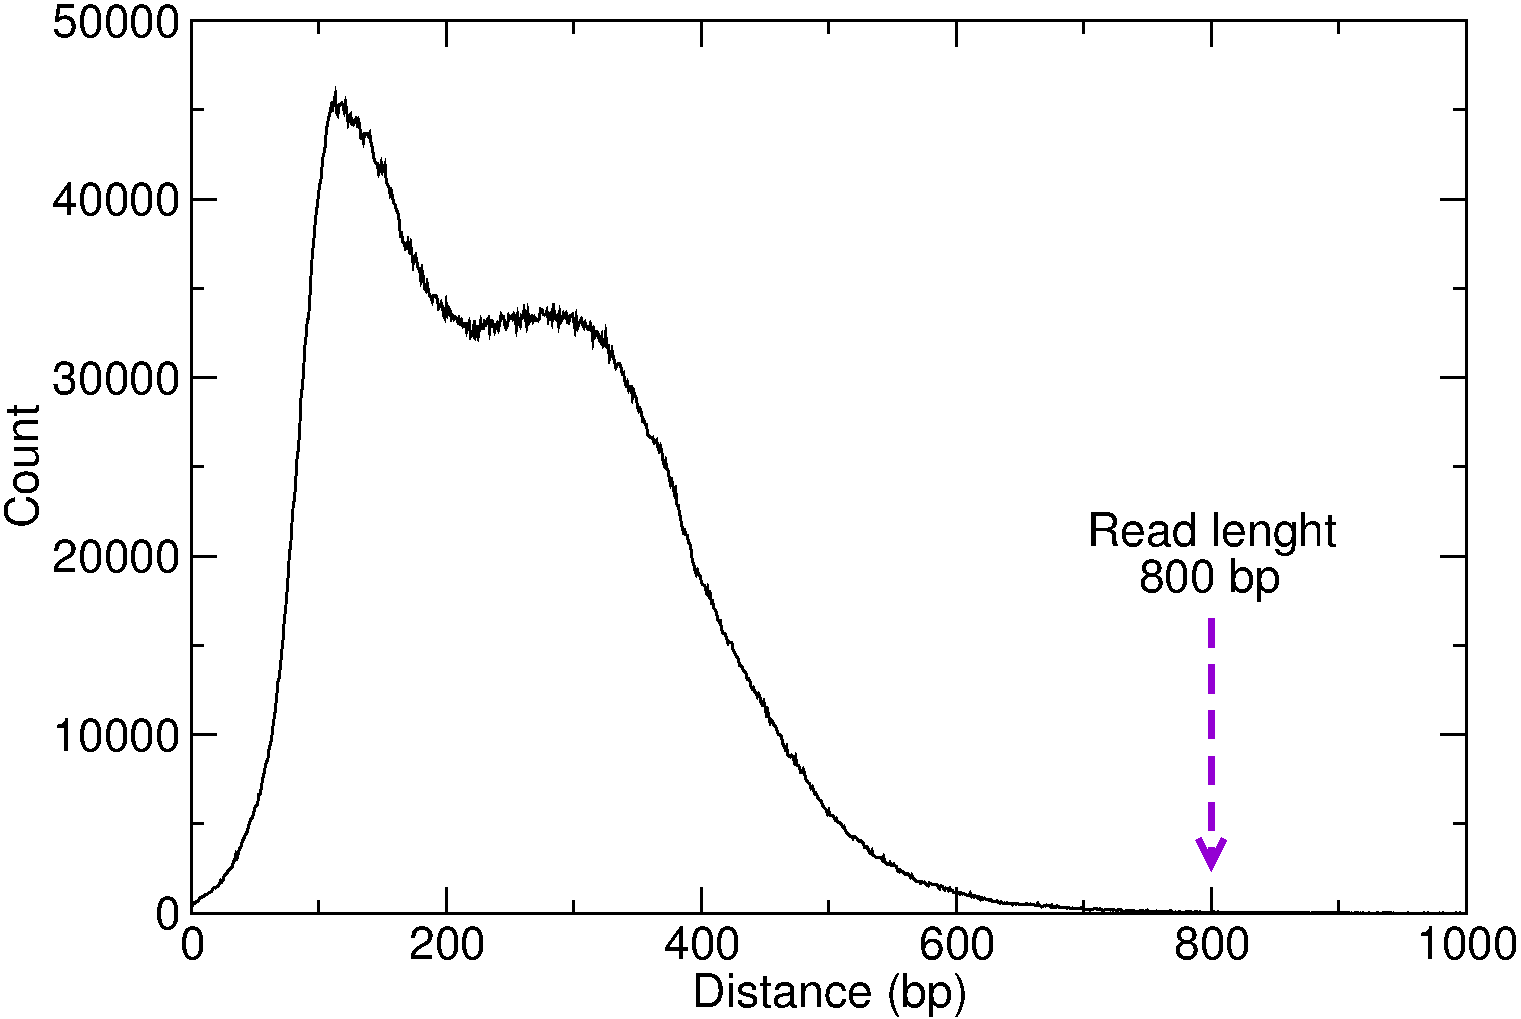
\includegraphics[width=8cm]{dangling}\\
where the graph has been made by summing the histogram of all
datasets, we can extimate the read length of 800bp.

Using the extimated read length we can apply a filter to the data in
order to remove part of the aligned reads which with good probability
don't belong to interaction and which are by-product of the sequencing
experiment. We filter out in particular the couples of reads which
belong to the same or the nearest-neighbour restriction fragment and
the reads which are dangling-ends and are located at a distance
less then the extimated read-length. After this filtering we
end up with the following number of chromosomal interactions:
\begin{verbatim}
SRR554454.sra:   1363227    SRR554455.sra:   1656343    SRR554456.sra:   1560418
SRR554457.sra:   5507976    SRR554458.sra:   2698946    SRR554459.sra:   2464849
SRR554460.sra:   3602954    SRR557710.sra:   5547465
\end{verbatim}

\section{Observations}
The distribution of interactions per site follows the typical Ori-TER copy
number variation as for a typical DNA sequencing experiment in \ecoli:

\vspace{.5cm}\hspace{2cm}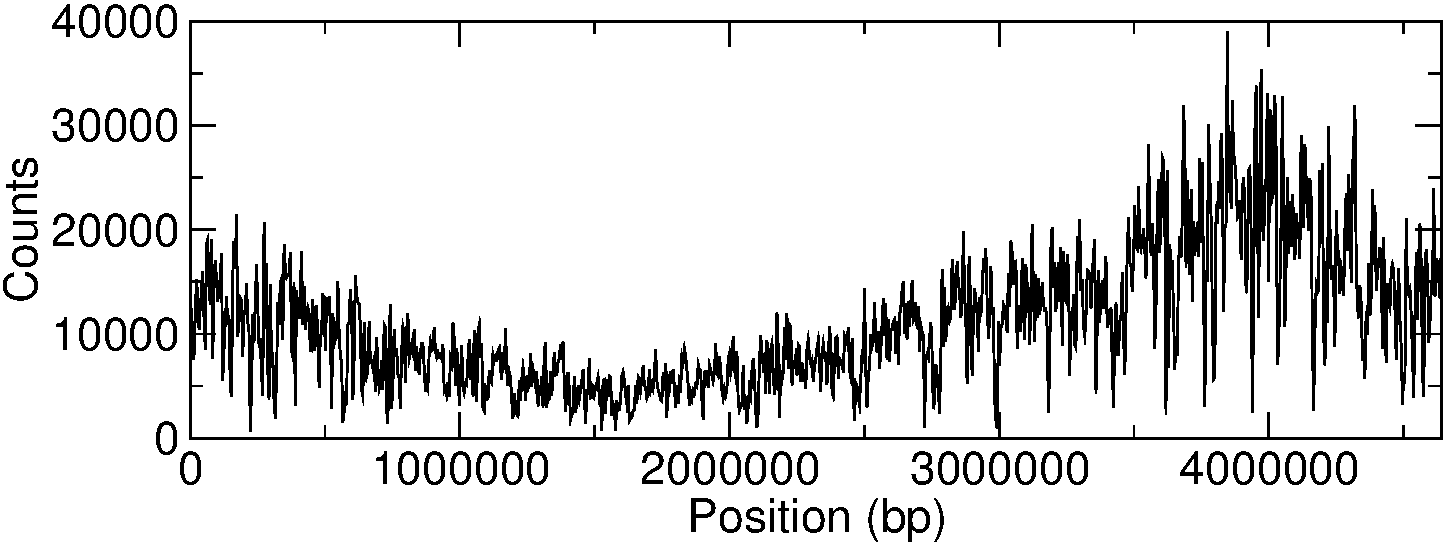
\includegraphics[width=12cm]{SRR554457ongenome}\\
the data comes from SRR554457 experiment, the bin is 1000bp, other
experiments show a similar trend. This indicates that a proper
normalization of the data is necessary.

Another interesting observable is the number of interaction in
function of the genomic distance. This is interesting because if it
defines a power law $p(s) \sim s^{-\alpha}$ then the exponent $\alpha$
can be connected to different polymer models as it has been done by
the Dekker group in a Science paper\cite{Lieberman2009}. We obtain the
following graph:

\vspace{.5cm}\hspace{2cm}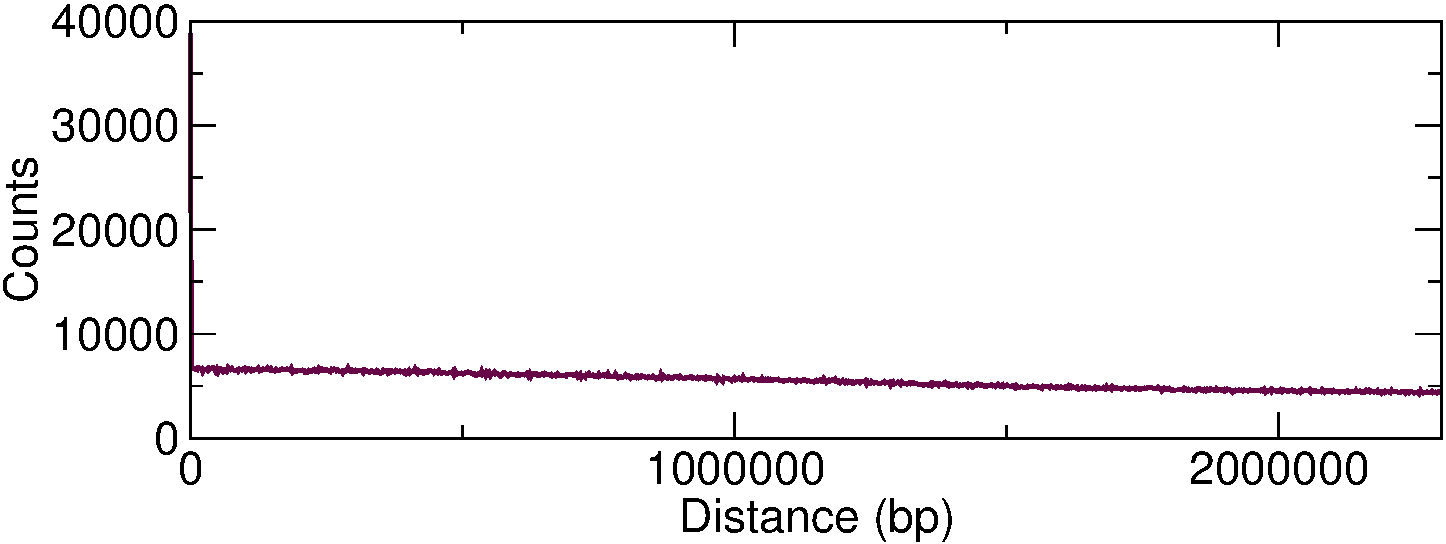
\includegraphics[width=12cm]{SRR554457dist}\\
which seems like an almost flat distribution. This would fit a random
gas model in which restriction fragments floating in a fluid randomly
ligates and form interactions, but it does not fit any polymer model.

We can make the contact map using the raw data, we obtain:

\vspace{.5cm}\hspace{2cm}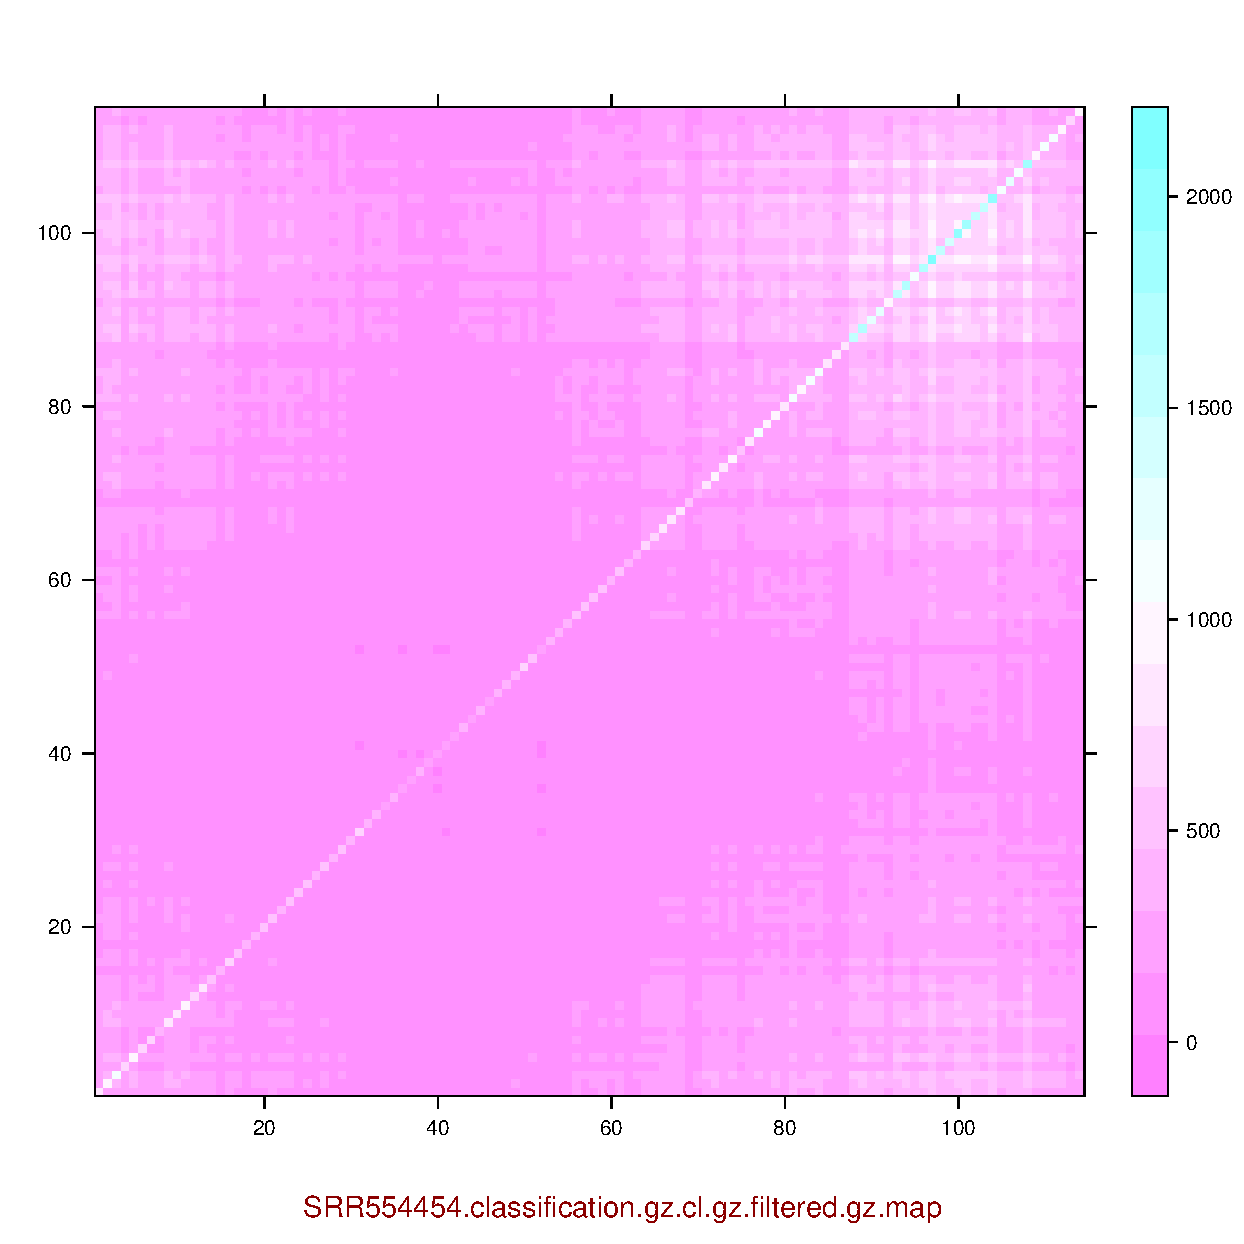
\includegraphics[page=1,width=12cm]{out}\\
with a bin size of 80000bp which can be reduced to 20000bp with still
decent results, here again the Ori-TER trend is dominating over the
interaction data.

We used the iterative correction algorithm\cite{Imakaev2012} to
eliminate the Ori-TER, as well as the other, biases. The basic idea of
this algorithm is that any experimental interaction matrix $O_{ij}$ is
in fact a real interaction matrix $T_{ij}$ bracketed by a
factorizable bias vector $B_i$ which depend on the genome position $i$:
\begin{equation}
O_{ij} = B_i T_{ij} B_j.
\end{equation}
The factorizable bias as well as the real interaction matrix can be
extracted from the data by using the iterative correction
algorithm. The rationale of removing this bias is that it mostly
depends by biological processes which are orthogonal from the
chromosome conformation (the copy number) and/or other systematic
errors. It is rationally clear that any real interaction in matrix
form should not be factorizable and thus would be left intact in the
process if it's signal is relevant in the dataset. We applied the
algorithm and we got the following bias vectors:

\vspace{.5cm}\hspace{2cm}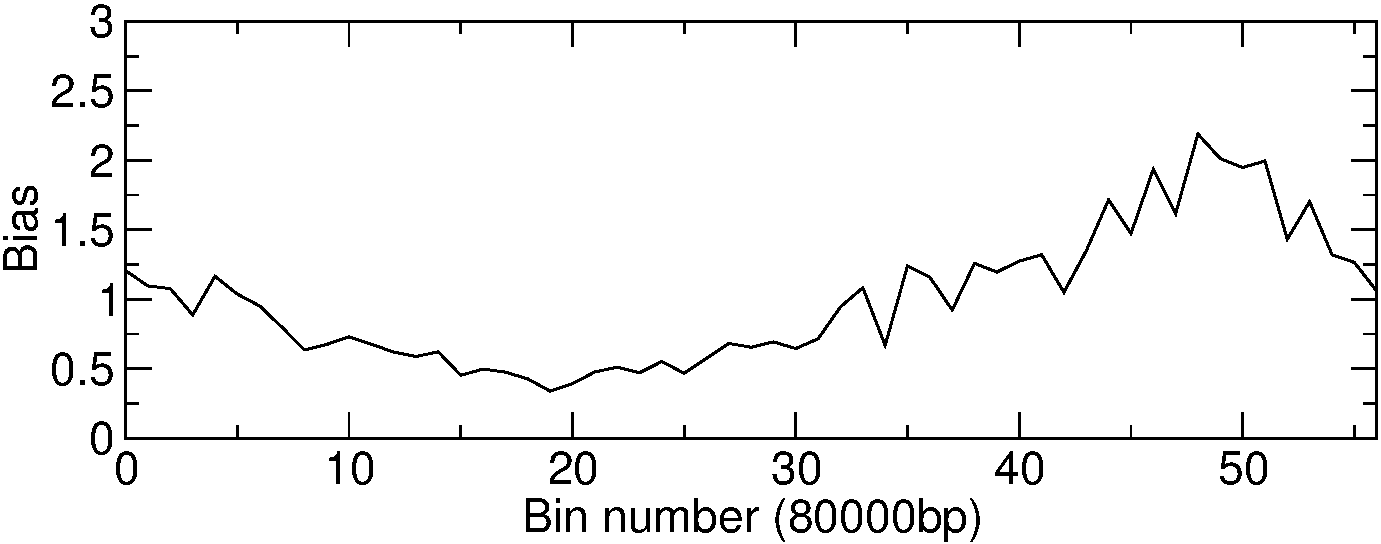
\includegraphics[width=12cm]{SRR554457bias}\\

After division, the interaction matrix becomes like this:

\vspace{.5cm}\hspace{2cm}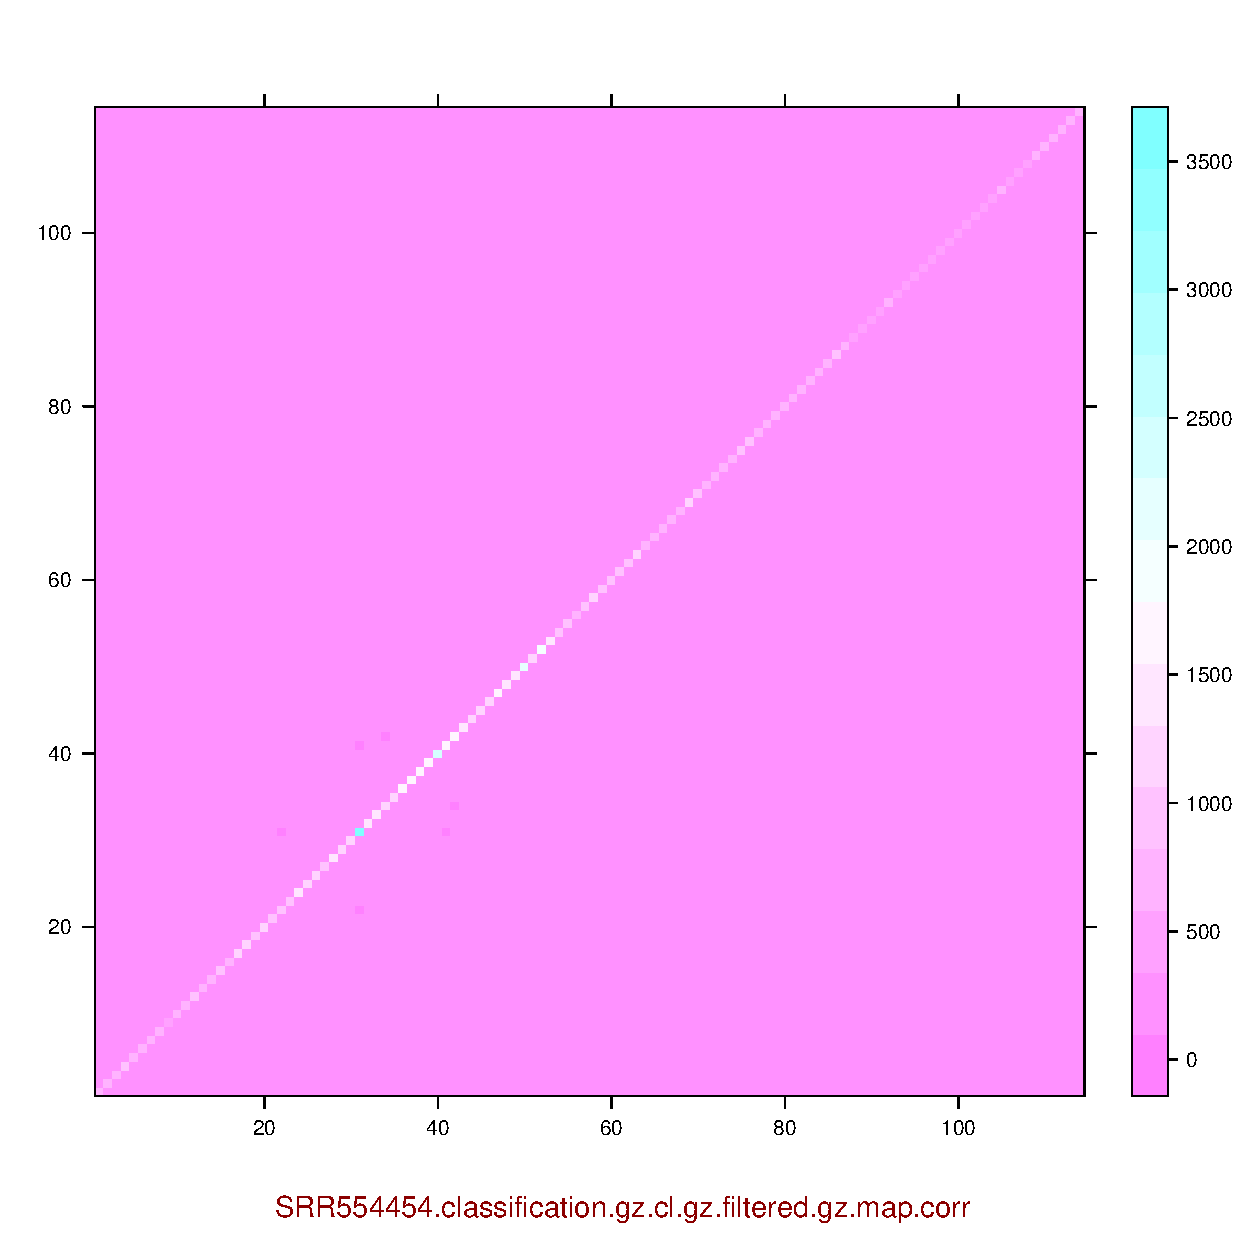
\includegraphics[page=1,width=12cm]{corr}\\

The code of the data analysis was written with the following
opensource tools: PERL (large file manipulation), Awk (counting),
Bash (prototyping), R (graphics) and Scilab (Matrix calculations).

\section{Analysis on Caulobacter}

The chromosome conformation capture have been performed also on
Caulobacter, another procariote, with a totally different technique
called 3C\cite{Umbarger2011} in Church group. While raw sequencing
data is not available for this paper, they provided a matrix of
interaction between restriction sites which did let us perform the
pipeline on at least the last part of the analysis.

The experiment of chromosome conformation capture was executed on
three biological replicates, with the following number of interaction
identified:
\begin{verbatim}
Replicate 1: 2111869 interactions
Replicate 2: 2417945 interactions
Replicate 3: 1996994 interactions
\end{verbatim}

A plot of the density of interactions in function of the position on
the genome gives us the following profile:

\vspace{.5cm}\hspace{2cm}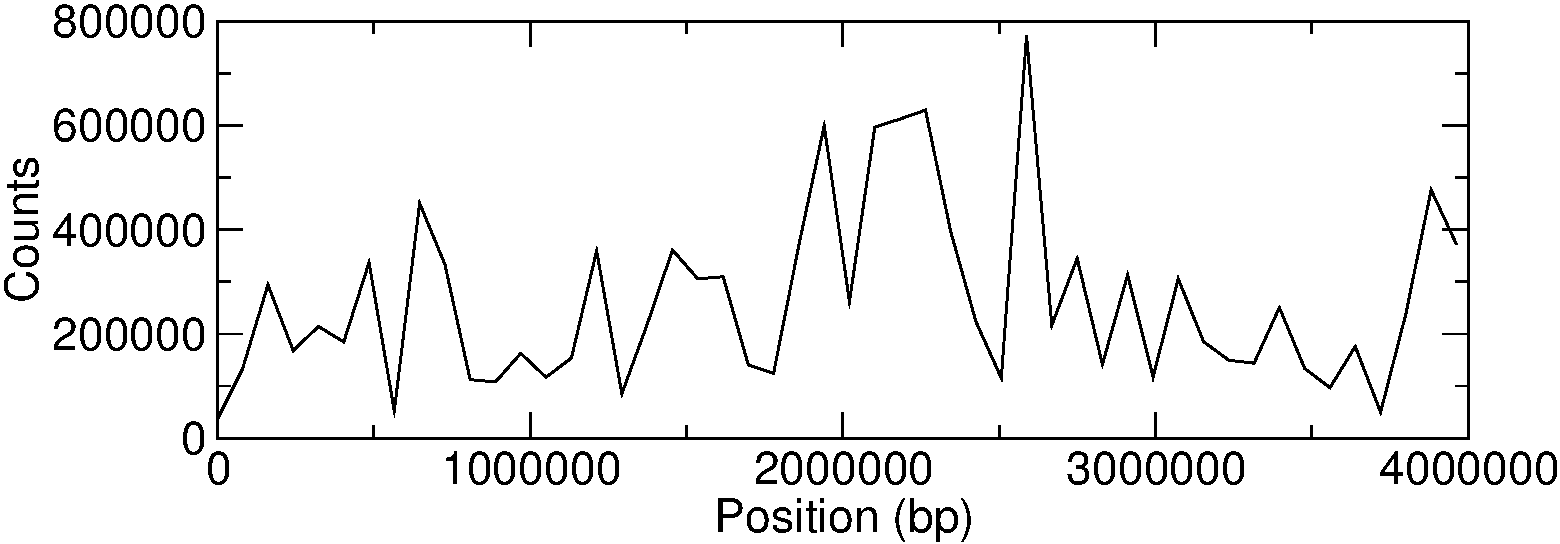
\includegraphics[page=1,width=12cm]{genocaulo}\\
which has been made by summing the data from all the
replicates and rebinning to 50 bins. Graphs for the single replicates
looks similar but more noisy. This graph shows a lot of variability in
function of genome cohordinate in the same way, if not even stronger,
as the \ecoli data.

In this case what is very different is the number of interactions in
function of the genomic distance $p(s) \sim s^{-\alpha}$ which in
this case is a power law as expected from polymer models:

\vspace{.5cm}\hspace{2cm}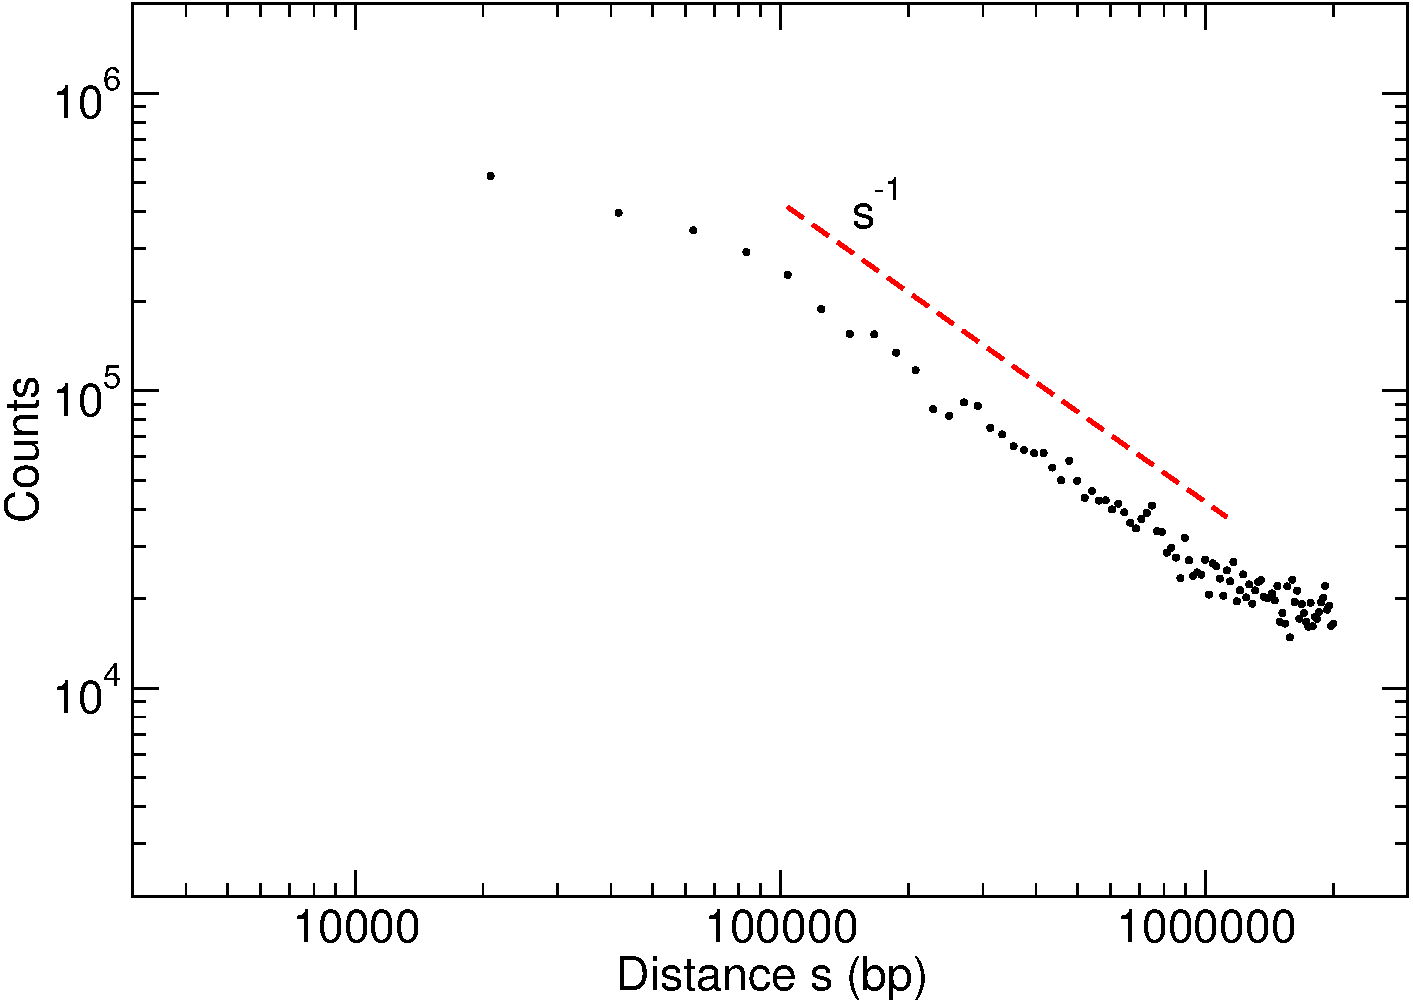
\includegraphics[page=1,width=12cm]{distcaulo}\\
where the parameter $\alpha = 1$ correspond to the one found on the
Human genome\cite{Lieberman2009}. In the Human case a fractal polymer
has been proposed as a fitting model.

The contact map of the rebinned raw data for the summed biological
replicates is the following:

\vspace{.5cm}\hspace{2cm}\includegraphics[page=4,width=12cm]{caulobacter/out}\\
which shows the elicoidal structer in which two arms of the chromosome
interact which each others. After the iterative correction we obtain
the following bin bias $B_j$:

\vspace{.5cm}\hspace{2cm}\includegraphics[page=1,width=12cm]{caulobacter/biascaulo}\\
and the following renormalized contact map:

\vspace{.5cm}\hspace{2cm}\includegraphics[page=4,width=12cm]{caulobacter/corr}\\
which shows a clear improvement after the elimination of the bias.

\bibliography{bd.bib}{}
\bibliographystyle{plain}

\end{document}
